\documentclass[12pt, a4paper]{article}

\usepackage[utf8]{inputenc}
%\usepackage[spanish]{babel}
\usepackage{amsmath}
\usepackage{amsfonts}
\usepackage{amssymb}
\usepackage{graphicx}
\usepackage{float}
\usepackage{listings}
\usepackage{multirow}

\usepackage[left=2cm,right=2cm,top=2cm,bottom=2cm]{geometry}

\author{5175: \'Angel Moreno \\ Tarea \# 5: Caracterización estructural de instancias}
\title{Optimizaci\'on flujo en redes}

\begin{document}
\maketitle

Se utiliza el generador de grafo \texttt{wheel\_graph} el consiste en generar un grafo donde tenga un nodo conectados a todos y los demas conectados en forma en circular, este tipo de grafo se uiliza comunmente cuando de un deposito o fuente se desea traladar o proporcionar algun material, energia, agua, etc. Las siguientes figuras muestran algunos ejemplos de instacias de un grafo con 16 nodos variendo la fuente y el sumidero para encontrar el flujo maximo utlizando el algoritmo \texttt{maximum\_flow}.


\begin{figure} [H] \centering
\includegraphics[scale=0.8]{G1}
\caption{Grafo con fuente 9 y sumidero 15.}
\label{fig: g1}
\end{figure}

\begin{figure} [H] \centering
\includegraphics[scale=0.8]{G2}
\caption{Grafo con fuente 15 y sumidero 14.}
\label{fig: g2}
\end{figure}

\begin{figure} [H] \centering
\includegraphics[scale=0.8]{G3}
\caption{Grafo con fuente 12 y sumidero 6.}
\label{fig: g3}
\end{figure}

\begin{figure} [H] \centering
\includegraphics[scale=0.8]{G4}
\caption{Grafo con fuente 12 y sumidero 8.}
\label{fig: g4}
\end{figure}

\begin{figure} [H] \centering
\includegraphics[scale=0.8]{G5}
\caption{Grafo con fuente 2 y sumidero 4.}
\label{fig: g5}
\end{figure}

\section{Resultados}

Se ejecuta el algoritmo de flujo m\'aximo un total de 30 r\'eplicas para medir su tiempo de ejecuci\'on, recordadndo que los distintos grafos tienen diferentes fuentes y sumideros. La figura \ref{fig: fig1} muestra los resultados, se observa qe los tiempos se comportan similares para los grafos del 2 al 5, muestras que le grafo 1 demoro mas tiempo que los demas.

\begin{figure} [H] \centering
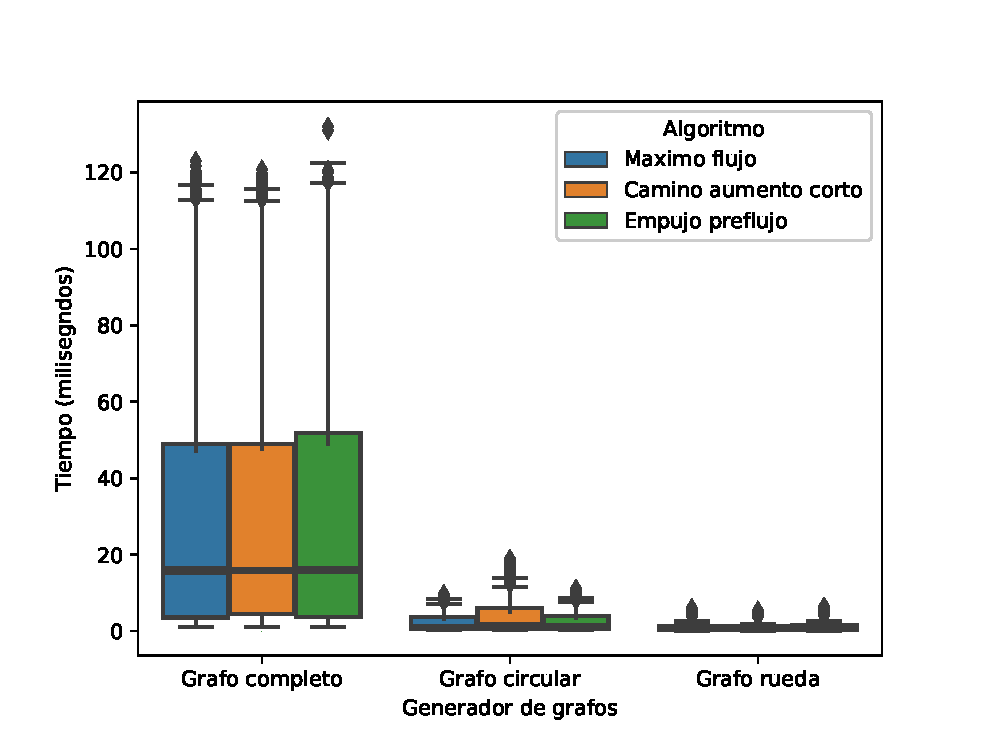
\includegraphics[scale=0.8]{figura1}
\caption{Efecto de las distintas instacias contra tiempo de ejecuci\'on.}
\label{fig: fig1}
\end{figure}

Esto se debe a las fuentes y sumideros escogidos, el cual en el primer grafo los vertices de fuente y sumideres estoy muy lejos esto implica mayor tiempo de ejecuci\'on, mientras los demas se ejecutan en menos tiempo. Se recomienda utilizar fuentes y sumideros tan alejados para menor tiempo de ejecuci\'on.

La figura \ref{fig: fig2} muestra el flujo maximo obtenido para cada grafo.

\begin{figure} [H] \centering
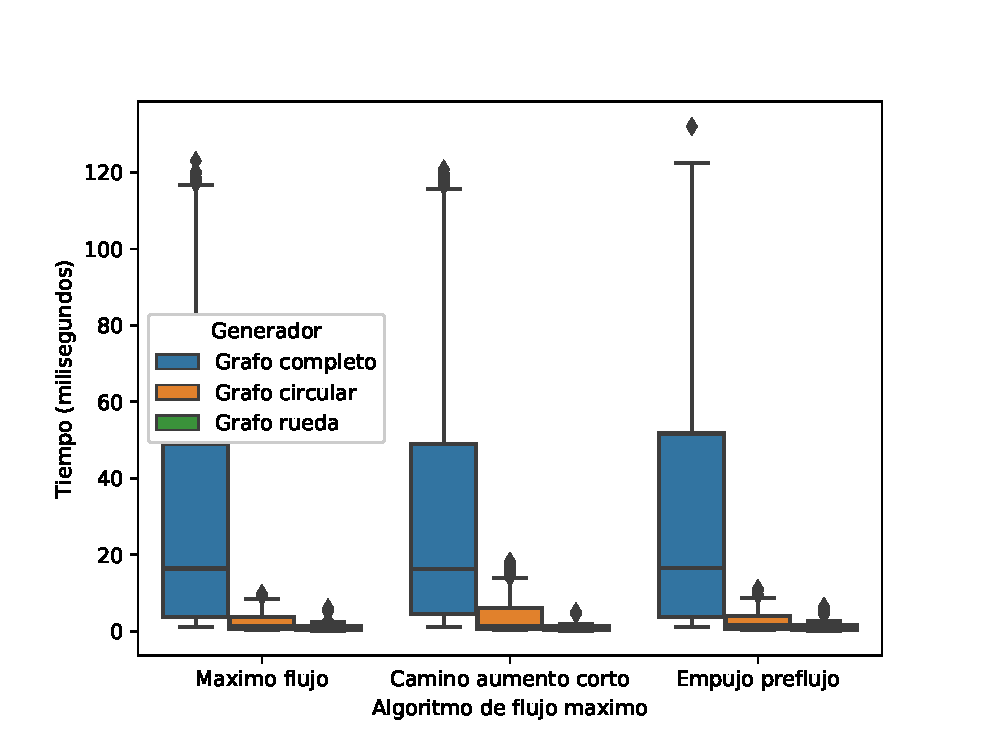
\includegraphics[scale=0.8]{figura2}
\caption{Efecto de las distintas instacias contra tiempo de flujo m\'aximo.}
\label{fig: fig2}
\end{figure}



\begin{thebibliography}{X}
\bibitem{elisa} \textsc{Schaeffer E.} \textit{Optimización de flujo en redes, 2019.} \\
\texttt{https://elisa.dyndns-web.com/teaching/opt/flow/}
\bibitem{lalo} \textsc{Kamada T.} \textit{An Algorithm for Drawing General Undirected Graphs} \\
\texttt{Information Processing Letters, 1988.}
\bibitem{lili} \textsc{Saus L.} \textit{Repository of Github, 2019.} \\
\texttt{https://github.com/pejli}
\end{thebibliography}


\end{document}